\chapter{Software}
Software pro elektronickou hru Logic byl napsán v jazyce C++. Bylo využito skutečnosti, že mikrokontrolér ESP32-PICO podporuje Arduino 
framework. Pro psaní softwaru bylo použito vývojové prostředí Visual Studio Code. \textcolor{red}{citace}%odkaz - citace

Pro programování inteligentních LED bylo využito již existující knihovny SmartLeds.h \textcolor{red}{citace}%odkaz - citace
Tato knihovna velmi usnadňuje softwarovou práci s těmito inteligentními LED. Obsahuje například funkci {\it show}, která umožní zobrazit 
nastavené barvy na všech LED připojených k jednomu pinu mikrokontroléru ESP32-PICO. 

\section{Funkce init}
Funkce {\it \_init\_} slouží pro inicializaci vstupně-výstupních pinů. Všechny piny, na kterých jsou připojena tlačítka, jsou nastaveny jako 
vstupní se zapnutým softwarovým pull-up rezistorem. Piny, na kterých jsou připojeny inteligentní LED, jsou nastaveny jako výstupní. Piny,
kterými je ovládáno připojení napájecího napětí jednotlivých částí inteligentních LED, jsou nastaveny jako výstupní a mají přednastavenou 
počáteční hodnotu. První část je zapnuta, zbylé 2 jsou vypnuty. Zbylým dvěma částem je napájení zapínáno až ve chvíli, kdy mají dané 
inteligentní LED svítit.

\begin{minipage}{\linewidth}
\begin{lstlisting}[frame=single,numbers=right,caption={Funkce pro úvodní inicializaci hardwaru.},label=lst:priklad.vypis.kodu.C,basicstyle=\ttfamily\small, keywordstyle=\color{black}\bfseries\underbar,]
void _init_ (){
    pinMode(LED_PIN_GAME, OUTPUT);
    pinMode(LED_PIN_TASK, OUTPUT);
    pinMode(LED_PIN_EVAL, OUTPUT);

    pinMode(SET_POWER_LEDS_1_TO_4, OUTPUT);
    pinMode(SET_POWER_LEDS_5_TO_7, OUTPUT);
    pinMode(SET_POWER_LEDS_8_TO_10, OUTPUT);

    pinMode(SW_ENTER, INPUT_PULLUP);
    pinMode(SW_RIGHT, INPUT_PULLUP);
    pinMode(SW_LEFT, INPUT_PULLUP);
    pinMode(SW_END, INPUT_PULLUP);
    pinMode(SW_NEW_GAME, INPUT_PULLUP);
    pinMode(SW_YELLOW, INPUT_PULLUP);
    pinMode(SW_ORANGE, INPUT_PULLUP);
    pinMode(SW_RED, INPUT_PULLUP);
    pinMode(SW_PURPLE, INPUT_PULLUP);
    pinMode(SW_BLUE, INPUT_PULLUP);
    pinMode(SW_GREEN, INPUT_PULLUP);

    digitalWrite(SET_POWER_LEDS_1_TO_4, POWER_ON); 
    digitalWrite(SET_POWER_LEDS_5_TO_7, POWER_OFF);
    digitalWrite(SET_POWER_LEDS_8_TO_10, POWER_OFF);
}
    \end{lstlisting}
    \end{minipage}

\section{Funkce ovládání tlačítek}
Zákmity tlačítek, které se dějí při stisku tlačítka, jsou řešeny hardwarových způsobem pomocí filtračních kondenzátorů. Proto tento probém
není řešen softwarově. Je ale možné, že hráč tlačítko drží po dobu delší, než trvá jeden programový cyklus. Došlo by tak k detekci více stisků.

Aby k této detekci nedocházelo, čeká se po detekci stisku na puštění tlačítka. Až poté je vykonáván příkaz. Tím je zaručeno, že se 
např. kurzor posune vždy jen o jedno pole. Pro zjednodušení tohoto zápisu byly vytvořeny funkce {\it is\_pressed(SW)} a {\it wait\_for\_btn\_release(SW)}.
Argumentem obou funkcí je pin tlačítka, na které se dotazuje/čeká. Funkce {\it is\_pressed} má návratovou hodnotu typu bool. Typ bool nabývá pouze 2 hodnot.
Těmito hodnotami jsou „true“\ = 1 (pravda) a „false“\ = 0 (nepravda). Pokud je tlačítko zmáčknuto, funkce vrátí „true“\, pokud tlačítko zmáčknuto není, 
funkce vrátí „false“\. Návratová hodnota je poté vyhodnocována v podmínce, zda je konkrétní tlačítko zmáčknuto. 

\begin{minipage}{\linewidth}
\begin{lstlisting}[frame=single,numbers=right,caption={Funkce pro detekci stisku tlačítka.},label=lst:priklad.vypis.kodu.C,basicstyle=\ttfamily\small, keywordstyle=\color{black}\bfseries\underbar,]
bool is_pressed(int btn){
    if(!digitalRead(btn))
        return true;
    return false;
}
\end{lstlisting}
\end{minipage}

\begin{minipage}{\linewidth}
\begin{lstlisting}[frame=single,numbers=right,caption={Funkce čekající na puštění tlačítka.},label=lst:priklad.vypis.kodu.C,basicstyle=\ttfamily\small, keywordstyle=\color{black}\bfseries\underbar,]
void wait_for_btn_release(int btn){
    while(!digitalRead(btn))
        delay(1);
}
\end{lstlisting}
\end{minipage} 

Tlačítka s barvami plní 2 funkce. Nejprve nastaví barvu dané LED a poté posunou kurzor o jedno pole vpravo. Tlačítka s šipkou posouvají kurzor daným směrem. 
Pro tyto 2 postupy vznikly funkce {\it set\_color(led, color)} a {\it shift\_cursor(led, direct, length)}.
Funkce {\it set\_color} má 2 argumenty. Jedním argumentem je barva LED, kterou má nastavit a druhým je řetězec LED, kde má tuto barvu nastavit.

\begin{minipage}{\linewidth}
\begin{lstlisting}[frame=single,numbers=right,caption={Ukázka funkce nastavující barvu inteligentním LED.},label=lst:priklad.vypis.kodu.C,basicstyle=\ttfamily\small, keywordstyle=\color{black}\bfseries\underbar,]
void set_color (led_t &LED, Colors COLOR){
    const int num_max = 32;
    switch (COLOR){
        case YELLOW:
        LED.leds[LED.pos] = Rgb{num_max, num_max, 0}; 
        break;
        case RED:
        LED.leds[LED.pos] = Rgb{num_max, 0, 0}; 
        break;
        case BLUE:
        ...
    } 
}    
\end{lstlisting}
\end{minipage} 

Funkce {\it shift\_cursor} posune kurzor vpravo, nebo vlevo, dle předaného argumentu. Pokud se kurzor nachází na konci herního řádku a je předán 
argument pro posun kurzoru vpravo, je pozice přepočítána tak, aby se kurzor posunul na začátek herního řádku. Pokud se kurzor nachází na začátku herního 
řádku a je předán argument pro posun kurzoru vlevo, je pozice přepočítána tak, aby se kurzor posunul na konec herního řádku. 

\begin{minipage}{\linewidth}
\begin{lstlisting}[frame=single,numbers=right,caption={Funkce posouvající kurzor.},label=lst:priklad.vypis.kodu.C,basicstyle=\ttfamily\small, keywordstyle=\color{black}\bfseries\underbar,]
void shift_cursor (led_t &LED, Direct DIR, int length){
    if((DIR == RIGHT) && 
      !((LED.pos + 1 + LINE_LENGTH - length) % LINE_LENGTH))
        LED.pos -= LINE_LENGTH - (LINE_LENGTH - length) - 1;
    else if(DIR == RIGHT)
        LED.pos += 1;
    else if((DIR == LEFT) && 
           (LED.pos == 0 || !(LED.pos % LINE_LENGTH)))
        LED.pos += LINE_LENGTH - (LINE_LENGTH - length) - 1;
    else if(DIR == LEFT)
        LED.pos -= 1;
}   
\end{lstlisting}
\end{minipage} 

\section{Zadání}
Vygenerování zadání a její následné uložení do inteligentních LED zajíšťují funkce {\it generate\_task(array, length, diff)} a {\it set\_task(leds, array, length)}.
Funkce generate task vygeneruje pomocí funkce {\it esp\_random} a matematické úpravy číslo od 0 do počtu barev. Každá barva je interpretována jiným číslem z tohoto 
rozsahu. Proměnná {\it diff} určuje, zda je může vygenerovat i černá (= mezera). Její hodnotu určuje stav přepínače. Proměnná {\it length určuje}, zda se vygeneruje zadání 
pro hru na 3 nebo 4 herní prvky. Její hodnota je také určována stavem přepínače. Zadání je uloženo do pole prvků, které je poté používáno pro vyhodnocení.

\begin{minipage}{\linewidth}
\begin{lstlisting}[frame=single,numbers=right,caption={Funkce pro vygenerování zadání.},label=lst:priklad.vypis.kodu.C,basicstyle=\ttfamily\small, keywordstyle=\color{black}\bfseries\underbar,]
void generate_task (Colors *task, int length, int diff){
    for(int i = 0; i < length; ++i)
        task[i] = Colors(esp_random() % (NUM_OF_COLORS - diff));
}      
\end{lstlisting}
\end{minipage} 

Funkce {\it set\_task} uloží hodnoty z pole, ve kterém je vygenerováno zadání, do inteligentních LED. Tam je uloženo a po zavolaní funkce {\it show} je ve správnou 
chvíli zobrazeno.

\begin{minipage}{\linewidth}
\begin{lstlisting}[frame=single,numbers=right,caption={Funkce pro vygenerování zadání.},label=lst:priklad.vypis.kodu.C,basicstyle=\ttfamily\small, keywordstyle=\color{black}\bfseries\underbar,]
void set_task(led_t &leds, Colors* array_task, int length){
    for (int i = 0; i < length; ++i){
        leds.pos = i;
        set_color(leds, array_task[i]); 
    } 
}      
\end{lstlisting}
\end{minipage}

\textcolor{red}{funkce evaluate - vyhodnocení} %evaluate - vyhodnocení

\chapter{Způsob ovládání elektronické hry}
DPS obsahuje 3 přepínače SW13, SW14 a SW15. Těmito přepínači si hráč volí způsob hry.

Přepínač SW15 slouží k volbě hry pro jednoho, nebo pro dva hráče. Pokud hráč umístí přepínač do pozice ON, hra se přepne
do módu pro dva hráče. Rozdíl mezi těmito variantami hry je popsán v následujících kapitolách, funkce dalších přepínačů taktéž.

\section{Hra pro jednoho hráče}
Tato verze hry pro jednoho hráče má stejná pravidla jako desková hra Logic. Funkci druhého hráče nahrazuje řídicí elektronika
- mikrokontrolér ESP32-PICO.

Po zapnutí DPS stikneme tlačítko "Nová hra"\ . V~této chvíli se vygeneruje zadání, které není vidět, a~první herní LED se 
rozbliká. Rozblikání herní LED značí pozici kurzoru. 
Kurzorem lze pohybovat pomocí tlačítek "Šipka vpravo"\  a~"Šipka vlevo"\ . Barvy herních LED se nastavují tlačítky ve spodní části 
DPS. Tato tlačítka jsou označena danými barvami.
Po zadání kombinace stiskneme tlačítko "Potvrdit tah"\ . Po stisku tlačítka proběhne vyhodnocení a~to se zobrazí na vyhodnocovacích LED. 
Červená barva ve vyhodnocení značí, že hráč má v barevné kombinaci stejnou barvu se zadáním na správné pozici. Žlutá barva znamená,
že hráč má v barevné kombinaci stejnou barvu se zadáním, ale na chybné pozici. Další barvy nejsou ohodnoceny. Pozice vyhodnocení
záměrně není shodná s pozicemi, kterých se hodnocení týká. Zleva jsou nejdříve umístěna všechna červená a až poté všechna žlutá 
hodnocení.

Po vyhodnocení se kurzor posune na první LED v~dalším řádku.
Po zadání správné kombinace barev a~jejich pozic se rozsvítí zadání a~hra je u~konce. Pro novou hru stiskneme tlačítko
"Nová hra"\  a~pro ukončení tlačítko "Konec"\ .
Po stisku tlačítka "Konec"\  zhasnou všechny herní, vyhodnocovací LED i~LED pro zadání. Poté je DPS připravena pro vypnutí
vypínačem.

Přepínač SW14 slouží pro nastavení, zda zadání obsahuje 3 nebo 4 barvy. Pokud hráč umístí přepínač do pozice ON, tak tím 
zvolí variantu hry na 3 barvy. Pohyb kurzoru se omezí na první 3 pole. Poslední pole se ignoruje a také nikdy nesvítí.

Přepínač SW13 slouží pro nastavení, zda zadání může nebo nesmí obsahovat mezeru. Pokud dá hráč přepínač do pozice ON, 
tak v zadání může být mezera. Není to ale nutností. 

\begin{figure}[!h]
    \begin{center}
        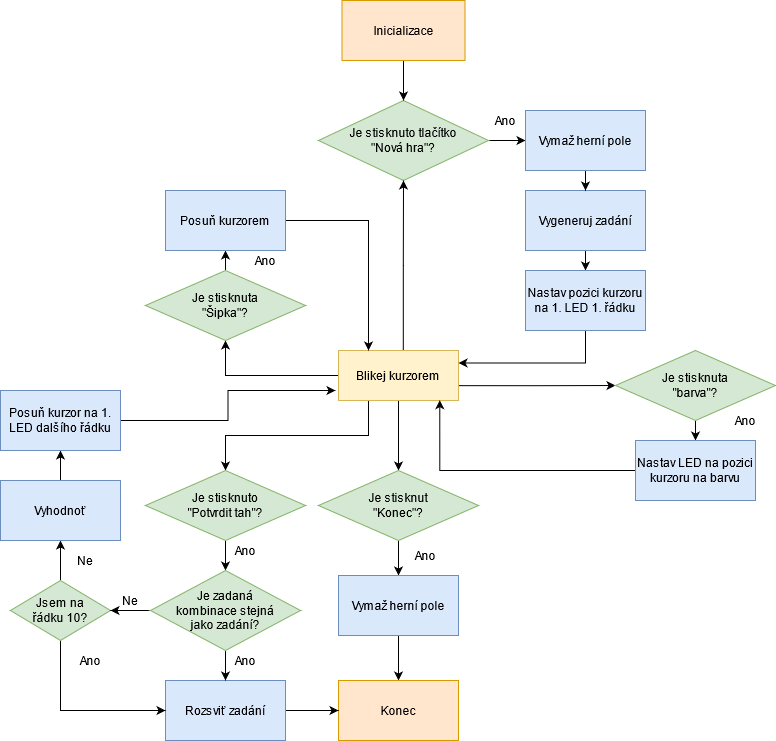
\includegraphics[scale=0.45]{obrazky/vyvojovy_diagram_1_hrac.png}
    \end{center}
    \caption[Vývojový diagram]{Vývojový diagram.}
    \end{figure}

\section{Hra pro dva hráče}
Varianta elektronické hry Logic pro dva hráče má totožná pravidla s deskovou hrou. Po spuštění hry a stisku tlačítka "Nová hra"\ .
bliká kurzor v poli inteligentních LED se zadáním. První hráč zadává barvy pomocí barevných tlačítek a v poli LED se pohybuje pomocí šipek 
interpretovanými tlačítky. Hráč zadání zakryje a stiskne tlačítko „Potvrdit tah“\ . 

Po stisku zadání zůstane svítit a kurzor se přesune na první herní pozici. Druhý hráč hádá zadanou kombinaci a tuto kombinaci 
navolí pomocí barevných tlačítek. Kurzorem může taktéž pohybovat pomocí šipek interpretovanými tlačítky. Po zadání kombinace 
druhý hráč stiskne tlačítko „Potvrdit tah“\  a kurzor se přesune na první pozici vyhodnocovacího pole. 

První hráč má v tuto chvíli aktivní pouze šipky a červené a žluté barevné tlačítko. Červenou barvu zadává jako první a 
indikuje jí, že některá barva druhého hráče je obsažena v zadání, a to na totožné pozici. Poté zadává žlutou barvu, kterou 
indikuje, že některá z barev prvního hráče je obsažena v zadání, ale na jiné pozici, než kam ji druhý hráč umístil. Vyhodnocení 
hráč záměrně neumisťuje na pozice, kterých se hodnocení týká. Zpravidla se zleva umisťují nejdříve všechna červená a až poté 
všechna žlutá hodnocení. 

Po dokončení hodnocení je opět kurzor posunut na první pozici dalšího řádku herního pole. Hra dále pokračuje obdobným způsobem.
Pokud druhý hráč nalezne správnou kombinaci, pak první hráč odkryje zadání pro možnou kontrolu a hra je u konce. Pro možnost další 
hry stiskne jeden z hráčů tlačítko „Nová hra“. Celé herní, vyhodnocovací pole i pole se zadáním je smazáno a kurzor je znovu posunut 
na první pozici pole se zadáním. 

\begin{figure}[!h]
    \begin{center}
        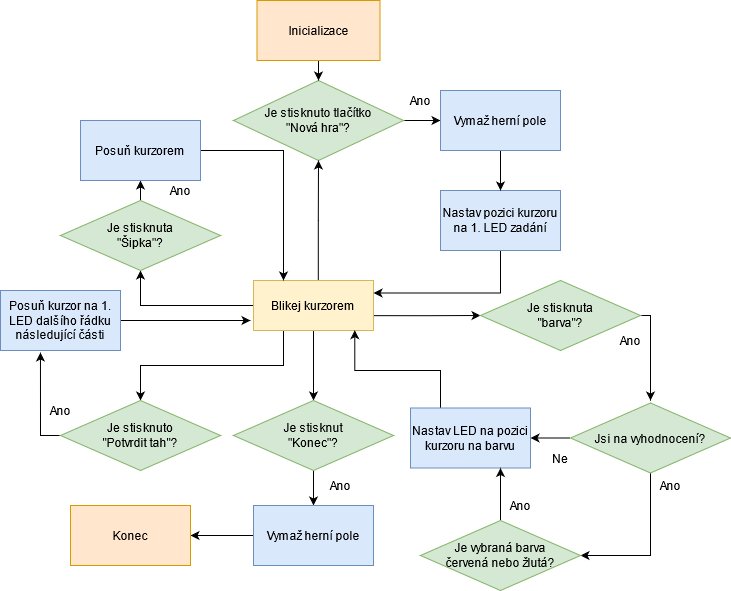
\includegraphics[scale=0.45]{obrazky/vyvojovy_diagram_2_hraci.png}
    \end{center}
    \caption[Vývojový diagram]{Vývojový diagram.}
    \end{figure}

\chapter{Krabička}
Krabička byla navržena v programu SolidWorks a vytištěna na 3D tiskárně. Krabička obsahuje 2 vyvýšené sloupky, do kterých jsou zalepeny 
matičky. Vnitřní a nižší jsou určeny pro přišroubování DPS pomocí montážních otvorů a šroubů M3. Vnější otvory jsou poté pro přišroubování 
vrchního krytu krabičky. V obou případech jsou použity šrouby M3 se zápustnou hlavou, protože mají podstatně nižší hlavičku, než šrouby klasické.

Krabička také obsahuje tzv. stříšku, která je také součástí deskové hry. Tato stříška slouží pro zakrytí zadání ve hře pro 2 hráče, kdy 
musí zadání svítit po celou dobu hry, aby druhý hráč byl schopen vyhodnocovat. 

\chapter{Kompletace}